\begin{blocksection}
\question Construct the following tree and save it to the variable \texttt{t}.

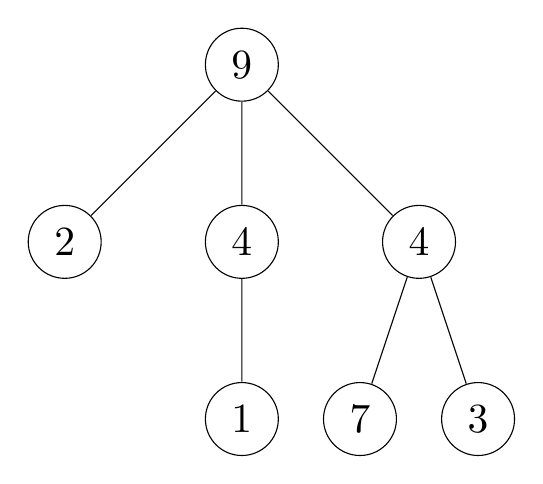
\begin{tikzpicture}[scale=1.5, transform shape]
\tikzstyle{level 2}=[sibling distance=10mm]
    \node [circle, draw] (z){$9$}
        child {node [circle, draw] (a) {$2$}}
        child {node [circle, draw] (d) {$4$}
            child {node [circle, draw] (g) {$1$}}
        }
        child {node [circle, draw] (b) {$4$}
            child {node [circle, draw] (e) {$7$}}
            child {node [circle, draw] (f) {$3$}}
        };
\end{tikzpicture}

\begin{solution}
\begin{lstlisting}
t = tree(9, [tree(2, []),
             tree(4, [tree(1, [])]),
             tree(4, [tree(7, []),
                      tree(3, [])])])
\end{lstlisting}
\end{solution}

\end{blocksection}
